\section{Background}

In this part we try to make the reader more familiar with the individual technologies and their
respective terms, that will be used throughout the thesis. Firstly we start by discussing the main
topic: Serverless Computing, we then will go on in more detail about \textit{Docker} and our
specific use case.

\subsection{Serverless Computing}

Serverless computing is a new emerging paradigm for deploying applications into the cloud. It gained
in popularity in recent years largely due to shift of enterprise application deployment in
containers and micro-services. Serverless Computing offers developers a simplified programming model
for creating cloud applications while minimising operational concerns. \cite{servprog}

The term “serverless” can be confusing, since physical server hardware is of course still needed in
order to run applications. The main point is that the application user or developer does not need to
manage scaling, plan for variable capacity or maintain any other aspect of the servers. All of this
is provided as a service from the cloud provider. \cite{wikiservcomp}

\subsubsection{Layers of Cloud Computing}

\begin{figure}[H]
  \centering
  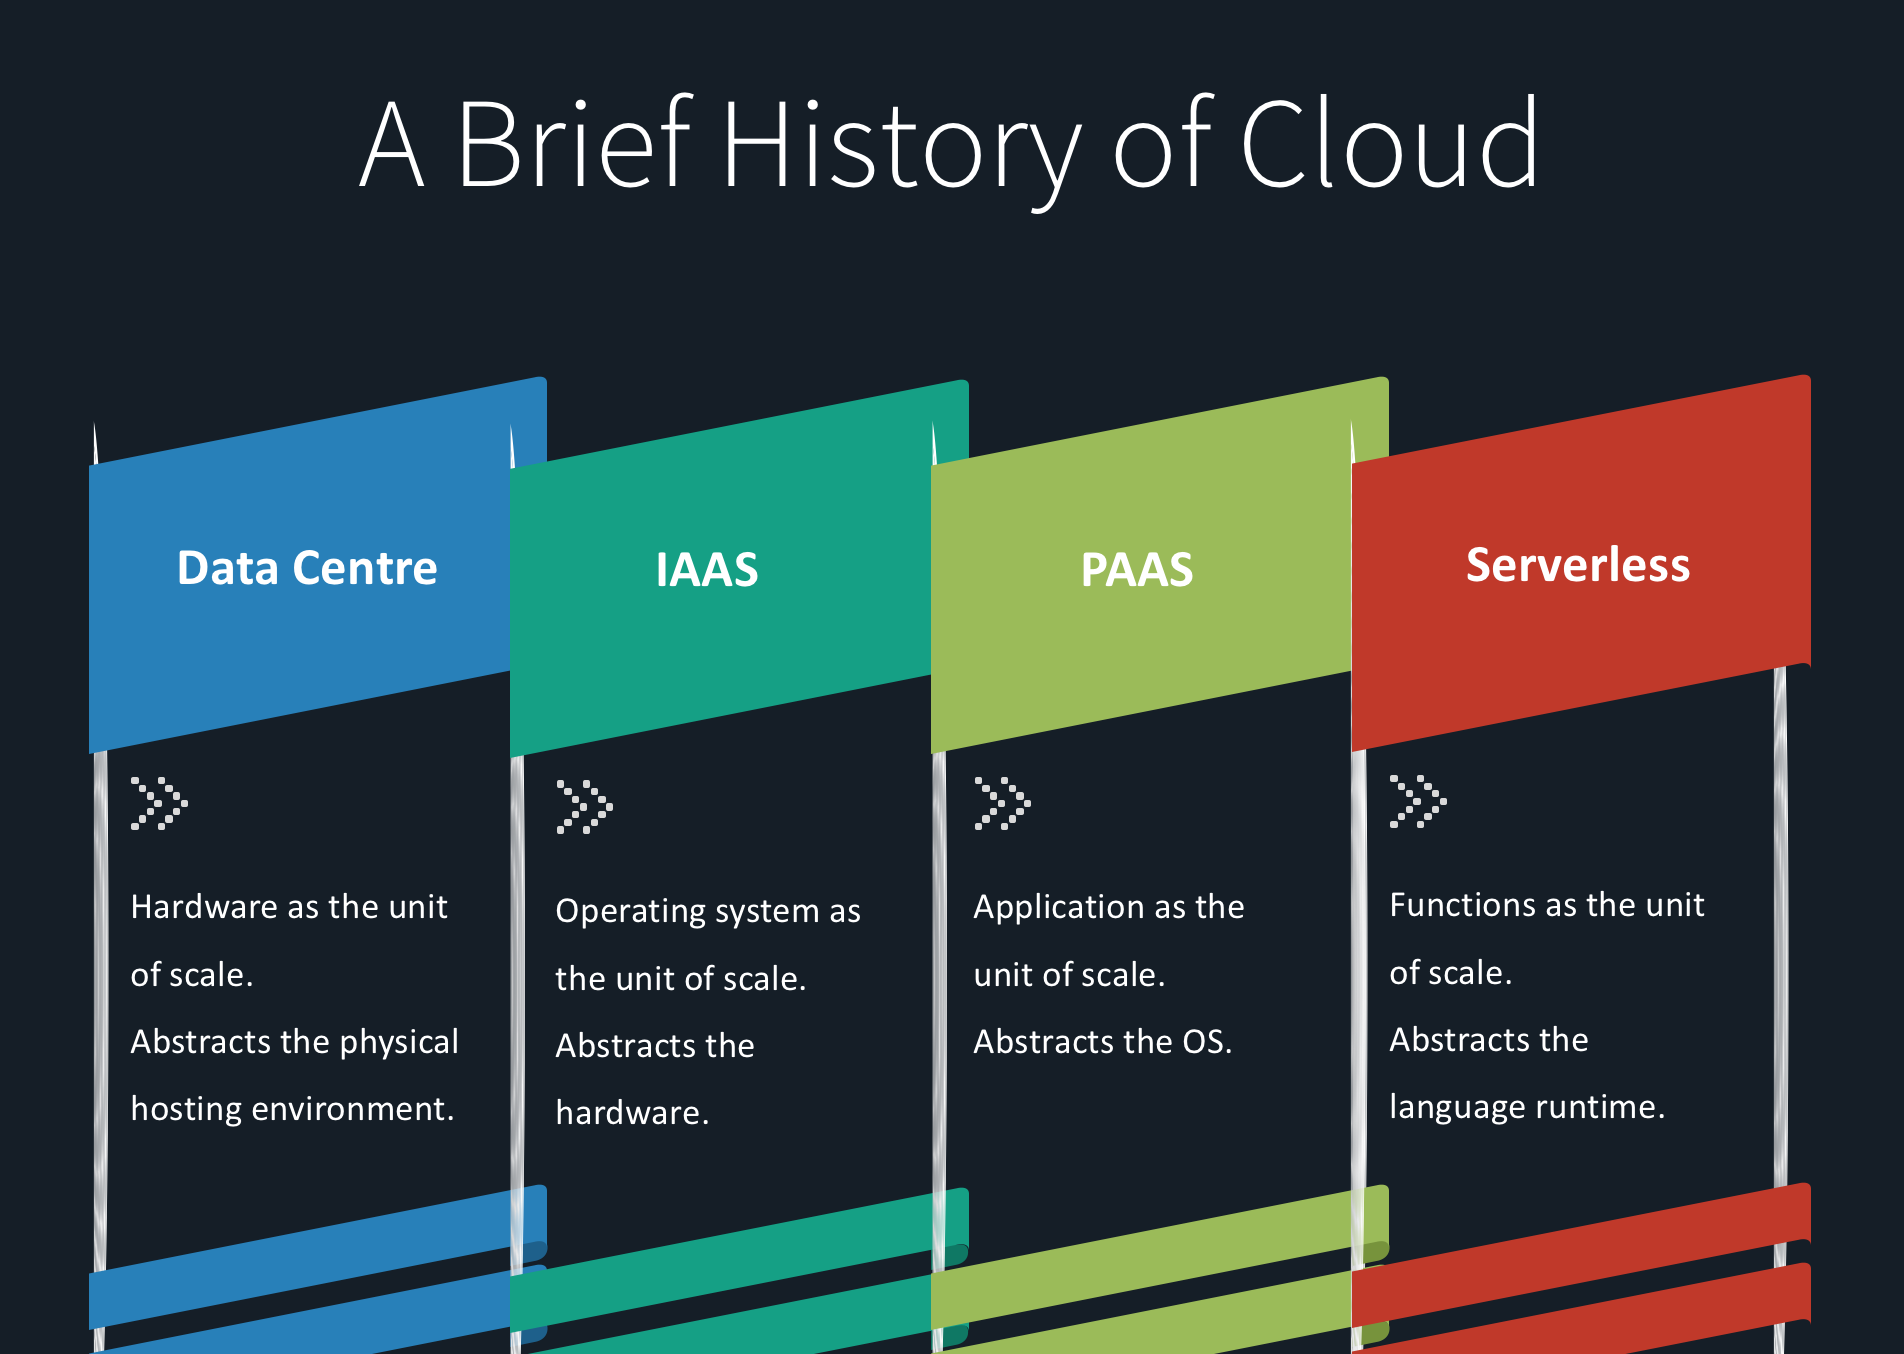
\includegraphics[height=20em]{cloud-history}
  \caption{History of cloud computing: going from Data Centre to IAAS, to PAAS, to finally Serverless (FAAS) \cite{layercloudcomp}}
\end{figure}

Historically, each new paradigm in the space of cloud computing has brought with it a new layer of
abstraction. First, there was the move from managing physical hardware in a data centre to being
able to rent infrastructure from a cloud provider. This layer, called IaaS (Infrastructure as a
Service), shifted the need for the customer to manage hardware infrastructure to the cloud
provider. This change also improved scalability as customers could now rent infrastructure on a
pay-as-you-go basis instead of paying for servers which would be idle most of the time.

With IaaS, the customer is still responsible for managing the setup of the rented infrastructure,
i.e. installing the necessary dependencies needed to run a given application. Naturally, the next
layer of abstraction is to provide the customer with an environment suited to run an application
without the need to manually install a programming language and any dependencies. This layer is
called PaaS (Platform as a Service). Using this layer of abstraction, the user does have to worry
neither about managing the underlying hardware nor about managing the operating system the
application is running on.

Now, in the era of serverless computing, there is yet again a new layer of abstraction. Called
FaaS (Function as a Service), this layer provides a runtime environment for a given language in
order to run functions. An application deployed in a FaaS environment consists of multiple
functions interacting with one another whereas in a PaaS environment, an application is deployed
as a single unit.
